\documentclass{jarticle}[2012/05/15]
\usepackage{graphicx}
\usepackage{misc}
\usepackage{listings,jlisting}
\begin{document}
\section{目的}
コンピュータの内部実装を学び、その動作原理と原始的な操作を習得する。
\par
\section{理論}
\subsection{機械語・アセンブリ言語}
アセンブリ言語はニーモックとオペランドからなる固定長の命令である。
\par
\subsection{レジスタ}
今回使用するH8マイコンは一つのレジスタを8,16,32ビットに使い分けることができる。\par
どの長さを使用するかはニーモックの接尾辞によって指定する。
\par
\pagebreak

\section{方法}
値をレジスタ内で計算し、メモリやLEDへ出力する。\par
今回は、LED8つを使って計算結果を確認する。\par
\subsection{実験1}
H'01000番地とH'01001番地のデータを8ビット加算してH'FEF10番地に格納する。
\subsection{課題2}
DATA1番地とDATA2番地の8ビットデータを16ビット加算してDATA3番地に格納する。
\subsection{実験3}
DATA1番地,DATA2番地の8ビットデータを符号付きソートする。
\subsection{実験4}
DATA1,DATA2,DATA3番地の符号無し8ビットデータから最大の値を選ぶ。
\subsection{実験5}
実験2のプログラムをサブルーチンに切り出す。
\subsection{実験7}
モールス信号で自分の名前をヘボン式ローマ字表記によって表現する。
\subsection{実験8}
ボタン入力のプログラムを作成する。
\subsection{実験9}
図\ref{src:void.c}のような簡単なCのプログラムから、アセンブラ・ソースを出力し、gcc -Sオプションでアセンブラソースを入手する。さらに、実行モジュールをobjdump -dで解析し、実際の動作を確認する。
\begin{figure}[htbp]
  {\scriptsize
   \listing{void.c}
   \caption{ソースコード void.c} \label{src:void.c}
  }
\end{figure}

\section{用具}
H8マイコンを搭載した中部大学製マイコン
\pagebreak

\section{結果}
\subsection{実験1}
実験1のアセンブラソースを以下に示す。実行結果はソース内に記述している(コメントは一部が右端で切れているが、見えない部分に重要なコメントはない)
{\scriptsize
   \lstinputlisting[label=src:01.src.txt, caption=01.src 課題1]{kadai01.src}
}
\pagebreak
\subsection{実験2}
実験2のアセンブラソースを以下に示す。実行結果はソース内に記述している(コメントは一部が右端で切れているが、見えない部分に重要なコメントはない)
{\scriptsize
   \lstinputlisting[label=src:02.src.txt, caption=02.src 課題2]{kadai02.src}
}
\pagebreak
\subsection{実験3}
図\ref{kadai3flow}のフローチャートにしたがってアセンブラを書いた。
\begin{figure}[htbp]
  \centering
  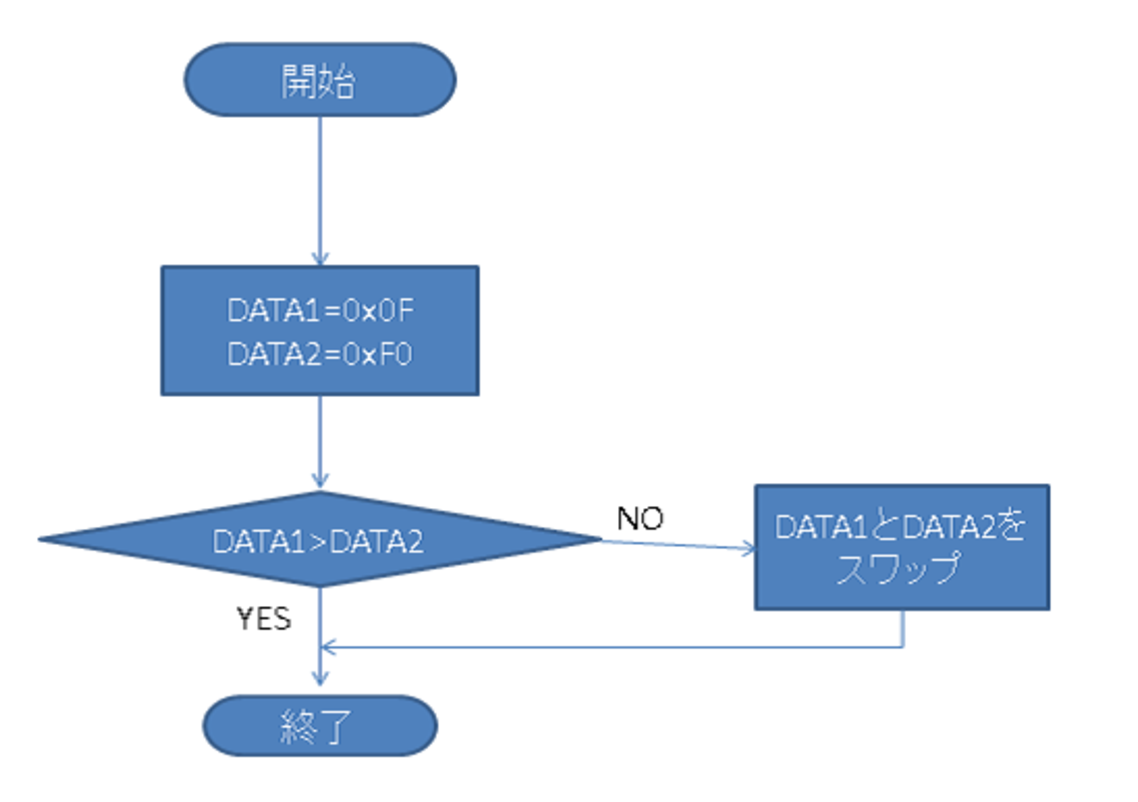
\includegraphics[width=8cm]{kadai3flow.eps}
  \caption{実験3フローチャート} \label{kadai3flow}
\end{figure}
実験3のアセンブラソースを以下に示す。実行結果はソース内に記述している(コメントは一部が右端で切れているが、見えない部分に重要なコメントはない)
{\scriptsize
   \lstinputlisting[label=src:03.src.txt, caption=03.src 課題3]{kadai03.src}
}
\pagebreak
\subsection{実験4}
実験4のアセンブラソースを以下に示す。実行結果はソース内に記述している(コメントは一部が右端で切れているが、見えない部分に重要なコメントはない)
{\scriptsize
   \lstinputlisting[label=src:04.src.txt, caption=04.src 課題4]{kadai04.src}
}
\pagebreak
\subsection{実験5}
\subsection{実験3}
図\ref{kadai5flow}のフローチャートにしたがってアセンブラを書いた。
\begin{figure}[htbp]
  \centering
  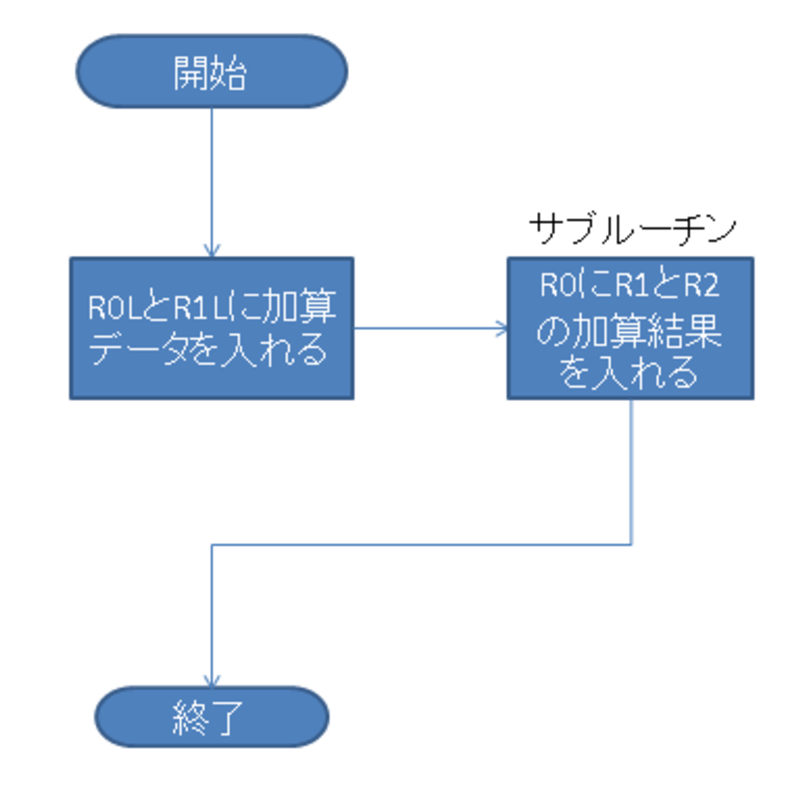
\includegraphics[width=8cm]{kadai5flow.eps}
  \caption{実験5フローチャート} \label{kadai5flow}
\end{figure}
実験5のアセンブラソースを以下に示す。実行結果はソース内に記述している(コメントは一部が右端で切れているが、見えない部分に重要なコメントはない)
{\scriptsize
   \lstinputlisting[label=src:05.src.txt, caption=05.src 課題5]{kadai05.src}
}
\pagebreak
\subsection{実験7}
実験7のアセンブラソースを以下に示す。動作内容はソース内に記述している(コメントは一部が右端で切れているが、見えない部分に重要なコメントはない)
{\scriptsize
   \lstinputlisting[label=src:07.src.txt, caption=07.src 課題7]{kadai07.src}
}
実行した結果、AOKIを符号化したものがLEDで点灯された。
\pagebreak
\subsection{実験8}
実験8のアセンブラソースを以下に示す。動作内容はソース内に記述している(コメントは一部が右端で切れているが、見えない部分に重要なコメントはない)
{\scriptsize
   \lstinputlisting[label=src:08.src.txt, caption=08.src 課題8]{kadai08.src}
}
実行した結果、ボタンを一部押すと対応するLEDが光り、ボタンを全部押すとLEDが点灯したままとなった。
\pagebreak
\subsection{実験9}
実行した結果得られたアセンブリソースから、mainサブルーチンのほか、各関数に対応するサブルーチンや、mainの前に実行されるサブルーチンなどが得られた。void.cから得られた結果を以下に挙げる。
{\scriptsize
   \lstinputlisting[label=src:void.s, caption=void.s 課題9]{void.s}
}
これをobjdump -dした結果から、mainのタグがついた部分を抜き出した。
\begin{lstlisting}[label=src:objdump, caption=objdumpの結果]
 080483b4 <main>:
 80483b4:	55                   	push   %ebp
 80483b5:	89 e5                	mov    %esp,%ebp
 80483b7:	b8 00 00 00 00       	mov    $0x0,%eax
 80483bc:	5d                   	pop    %ebp
 80483bd:	c3                   	ret    
 80483be:	90                   	nop
 80483bf:	90                   	nop
\end{lstlisting}

\section{考察}
\subsection{実験1}
この実験では実際にメモリに値が格納されているかどうかが分からないため、不完全なものとなっている。メモリの値を一度レジスタに読みだしたほうが好ましい。
\subsection{実験2}
実験1と同様、レジスタにメモリの値を読みだしてからLEDを点灯させるのが望ましい。
\subsection{実験3}
このとき、符号の有無を意識せず行ったため、FFが01よりも小さいという結果になり戸惑った。FFは先頭ビットが符号の役割を果たすため、実質-1である。\par
実際にはスワップを行わずそのままDATA1とDATA2番地に格納するのが好ましい。しかし今回のプログラムではDATA1とDATA2にそのまま書き込むことができない。これは機器の制限によるものである。したがって今回は「レジスタの値を入れ替えた」だけで満足とする
\subsection{実験4}
今回はスワップが必要ないため、実験4に比べて一つ一つの処理は簡略化できた。
\subsection{実験5}
メインルーチンの末尾にループがない場合、止まってしまった。
\subsection{実験7}
音と音の間を2拍、字と字の間を3拍として行った。関数への値受け渡しは特殊だが、サブルーチン呼び出しの処理をjsr命令がほとんど負担しているため、アセンブラでもCの関数とほぼ同じようにサブルーチンが使えることがわかった(ただし、メインルーチンの末尾にループが必要)。
\subsection{実験8}
CPUを停止させる方法が見つからなかったため、ループを用いて停止を表現した。
\subsection{実験9}
アセンブラソースおよびobjdump -dの結果から、main関数では、returnに渡した値(EXIT\_SUCCESS)をあるレジスタに入れたあと、retで脱出していることが分かった。これは他のCプログラムの関数呼び出しでも同様だった。ここからC言語のmain関数を含む基本的な関数呼び出しがアセンブラのサブルーチン呼び出しと同様だということが分かった。

\end{document}